\usepackage[numbers]{natbib}
\usepackage{algorithm}
\usepackage[noend]{algpseudocode}
\usepackage{adjustbox}
\makeatletter
\let\OldStatex\Statex
\renewcommand{\Statex}[1][3]{%
  \setlength\@tempdima{\algorithmicindent}%
  \OldStatex\hskip\dimexpr#1\@tempdima\relax}
\makeatother
% setup todo package and make compatible with tikz
\usepackage{todonotes}
% bug fix for `todonotes` vs `tikz` externalize
\usepackage{letltxmacro}
\LetLtxMacro{\oldmissingfigure}{\missingfigure}
\renewcommand{\missingfigure}[2][]{\tikzexternaldisable\oldmissingfigure[{#1}]{#2}\tikzexternalenable}
\LetLtxMacro{\oldtodo}{\todo}
\renewcommand{\todo}[2][]{\tikzexternaldisable\oldtodo[#1]{#2}\tikzexternalenable}

% list of abbreviations
\usepackage{longtable}
\usepackage[acronym, xindy, shortcuts, indexonlyfirst]{glossaries}

% better references
\usepackage[nameinlink, capitalise]{cleveref}
% TODO: maybe overload abbreviations for chapter, figure etc.

\usepackage{lipsum}

% Some useful macros for special formatting. % This doesn't make things
% shorter. It is just a form of typing things to make it easier to change it at
% a later point in time.

% variable names
\newcommand{\vname}[1]{\emph{#1}}
% real numbers
\newcommand{\argmax}{\operatornamewithlimits{argmax}}
\newcommand{\argmin}{\operatornamewithlimits{argmin}}
\newcommand{\reals}{\ensuremath{\mathbb{R}}}
\newcommand{\naturals}{\ensuremath{\mathbb{N}}}
\newcommand{\sspace}{\ensuremath{\mathcal{S}}}
\newcommand{\aspace}{\ensuremath{\mathcal{A}}}
\newcommand{\ospace}{\ensuremath{\mathcal{O}}}
\newcommand{\tdist}{\ensuremath{\mathcal{T}}}
\newcommand{\odist}{\ensuremath{\mathcal{Z}}}
\newcommand{\reward}{\ensuremath{\mathcal{R}}}
\newcommand{\bspace}{\ensuremath{\mathcal{B}}}
\newcommand{\oof}{\ensuremath{\mathcal{O}}}
\newcommand{\qfunction}{$Q$-function\xspace}
\newcommand{\chrond}{\delta}
\newcommand{\pomdpsjl}{\emph{POMDPs.jl}\xspace}
\newcommand{\mode}{\text{mode}\xspace}
\newcommand{\sml}{\ensuremath{s_\text{ml}}}

\newcommand{\ie}{i.e.\ }
\newcommand{\eg}{e.g.\ }
\newcommand{\cf}{c.f.\ }
\newcommand{\appdata}{PRO$\_$\NummerDerArbeit$\_$\NachnameDesStudenten}

% TODO: example of a rotate figure, maybe helpful for the appendix
%  \begin{figure}[ht]
%    \begin{adjustbox}{addcode={\begin{minipage}{\width}}{\caption{%
%    \todo[inline]{Describe and fix scaling and font}
%        }\end{minipage}},rotate=90,center}
%        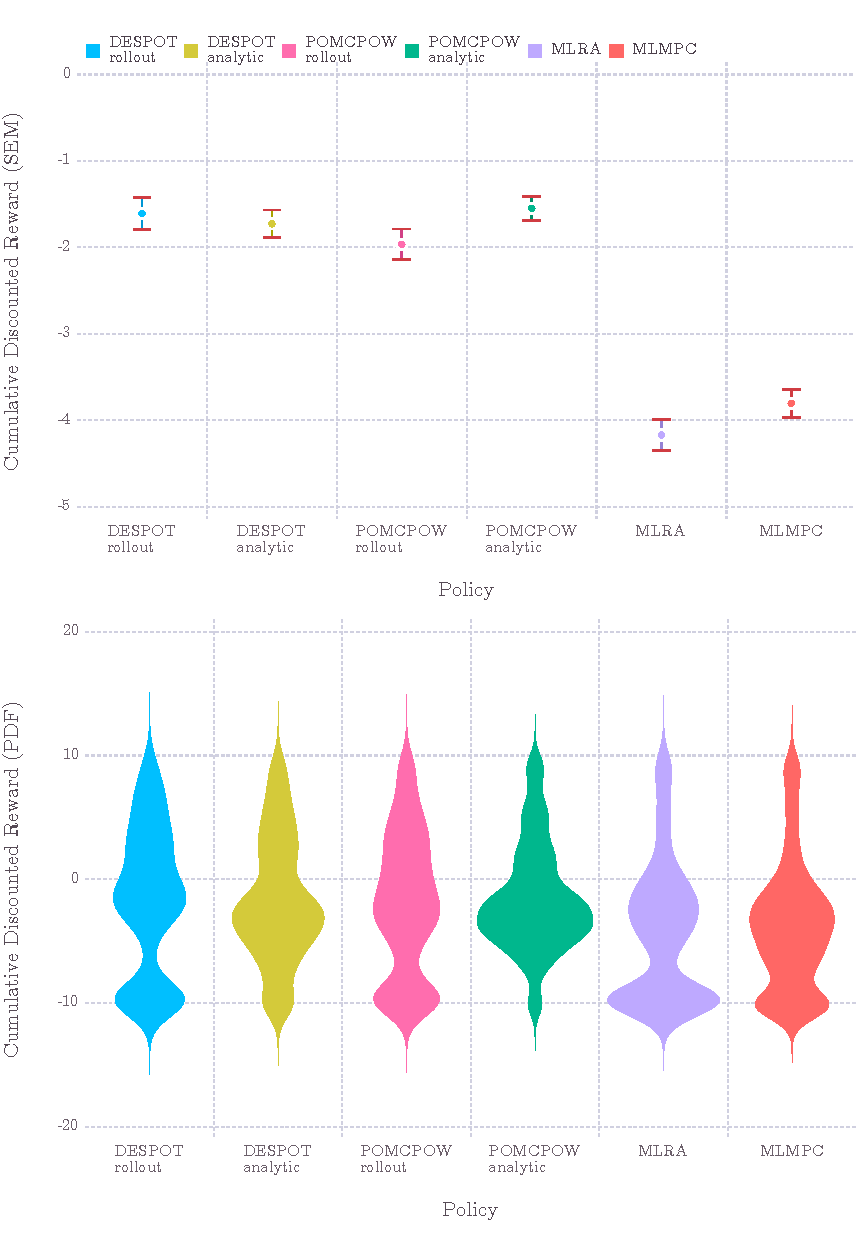
\includegraphics[scale=1]{roomba_plots/lp_value_eval_plot.pdf}
%    \end{adjustbox}
%  \end{figure}
